\documentclass{article}[12pt]
\usepackage{graphicx}
\usepackage{amsmath,amssymb}
\usepackage{tikz}
\usepackage{xepersian}
\settextfont[Scale=1]{IRXLotus}
\setlatintextfont[Scale=0.8]{Times New Roman}

\DeclareRobustCommand{\bbone}{\text{\usefont{U}{bbold}{m}{n}1}}

\DeclareMathOperator{\EX}{\mathbb{E}}% expected value


\title{  \includegraphics[scale=0.35]{../../Images/logo.png} \\
    دانشکده مهندسی کامپیوتر
    \\
    دانشگاه صنعتی شریف
}
\author{استاد درس: دکتر محمدحسین رهبان}
\date{بهار ۱۴۰۰}



\def \Subject {
تمرین چهارم
}
\def \Course {
درس یادگیری ماشین
}
\def \Author {
نام و نام خانوادگی:
امیر پورمند}
\def \Email {\lr{pourmand1376@gmail.com}}
\def \StudentNumber {99210259}


\begin{document}

 \maketitle
 
\begin{center}
\vspace{.4cm}
{\bf {\huge \Subject}}\\
{\bf \Large \Course}
\vspace{.8cm}

{\bf \Author}

\vspace{0.3cm}

{\bf شماره دانشجویی: \StudentNumber}

\vspace{0.3cm}

آدرس ایمیل
{\bf \Email}
\end{center}


\clearpage
 
\section{سوال ۱}
\subsection{الف}
 خب میبایست با استفاده از پرسپترون عملگرهای 
 NAND 
 و 
 NOR
 را پیاده سازی کنیم که بهتر است اول جدول آنها رو بکشیم. 
 \begin{LTR}
 \begin{table}[h]
 \centering
\begin{tabular}{|c|c|c|c|c|c|}
\hline
$x_1$ & $x_2$ & OR & AND & NOR & NAND \\ \hline
$-1$ & $-1$ & $-1$ & $-1$  & $1$   & $1$    \\
$-1$ & $1$  & $1$  & $-1$  & $-1$  & $1$    \\
$1$  & $-1$ & $1$  & $-1$  & $-1$  & $1$    \\
$1$  & $1$  & $1$  & $1$   & $-1$  & $-1$  
\\\hline
\end{tabular}
\end{table}
\end{LTR}

در اینجا برای فهم بهتر دو نمودار را رسم میکنیم:
\begin{center}
\includegraphics[scale=0.75]{diagram-20210422.pdf} 
\end{center}


نمودار سمت چپی برای NAND است و سمت راستی برای NOR
.
حال باید وزن هایی را پیدا کنیم که مقادیر ما در آن به درستی مدل شوند پس داریم:

\begin{equation}
y^{i} = sgn(w^T x^{i}+b) = sgn(w_1 x_1 + w_2 x_2 + b)
\end{equation}

برای مدل NOR میتوان وزن ها و مقادیر زیر را پیشنهاد داد:

\begin{equation}
y = (-1) x_1 + (-1) x_2 -0.5
\end{equation}

و برای مدل 
NAND
نیز میتوان مقادیر زیر را پیشنهاد داد:

\begin{equation}
y = (-1) x_1 + (-1)x_2 +0.5
\end{equation}
\clearpage
\subsection{ب}
فکر میکنم منظور از سوال این است که بتوانیم تشخیص دهیم که یک مدل چندلایه پرسپترون به چه صورت است و چگونه کار میکند و غیره. پس از کوچکترین سازه ها شروع کرده و به ترتیب جلو میرویم. 
ابتدا مشخص است که لازم داریم ۴ پرسپترون در لایه اول برای تشخیص بزرگتر کوچکتر بودن های زیر درست کنیم:

\begin{equation}
x>y; x<y;y<z;y>z
\end{equation}

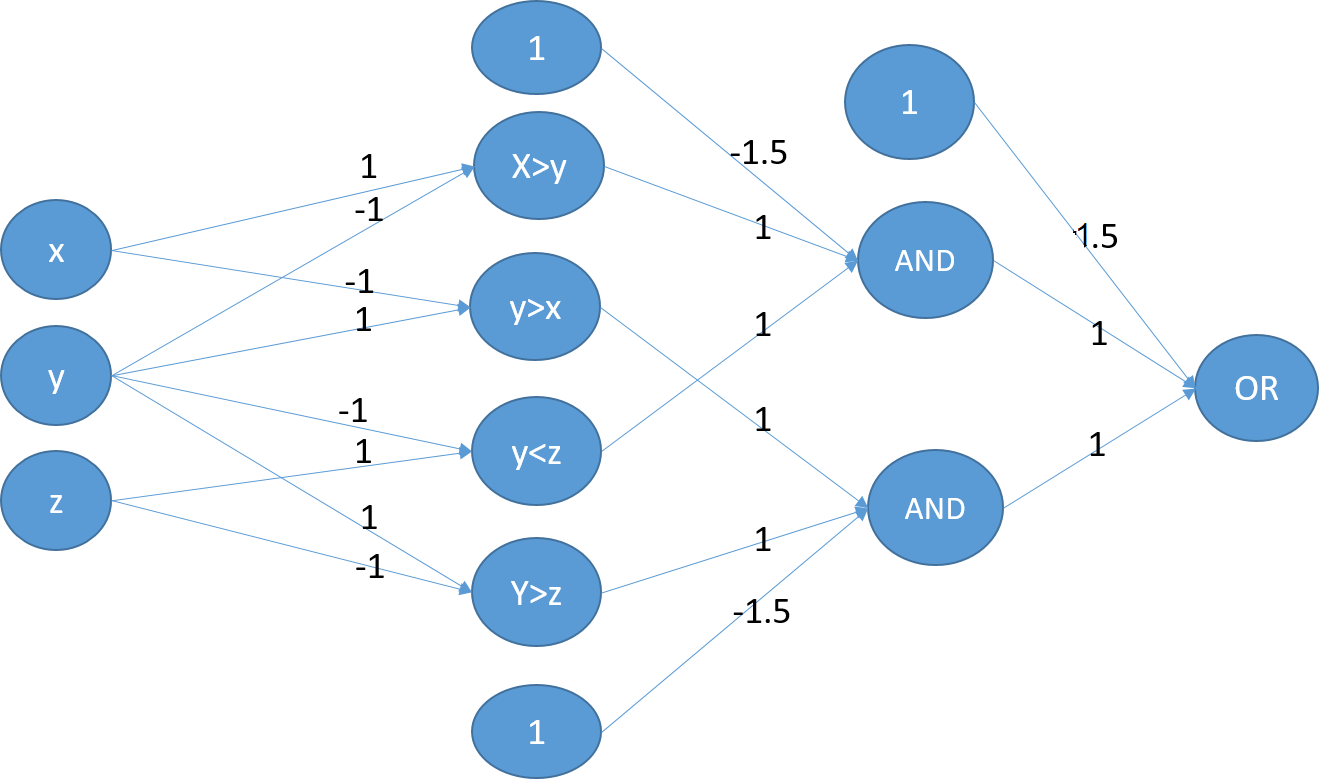
\includegraphics[scale=0.5]{NeuralNetwork.png} 

سپس با توجه به شکل دو عدد گیت AND
و یک عدد گیت 
OR 
در نهایت لازم هستند که به سادگی تمام با پرسپترون قابل پیاده سازی هستند. 

البته بهتر می بود که یک عدد ۱ در لایه اول میگذاشتم و از آن یک به هر دو AND وصل میکردم که دو خط وصل میشد و وزن هر دو 
$-1.5$
میبود اما به علت این که خط های موجود در شکل پیچیده و کمی تو در تو میشد دو عدد ۱ که نشان دهنده بایاس میباشد رسم کرده ام. 

\clearpage
\section{سوال ۲}

\subsection{الف}
فرض سوال
\begin{equation}
x_1 = 2 , w_1 = 1,x_2 = -1,w_2 = 3
\end{equation}


خب در ابتدا شکل را بصورت تابع دربیاوریم و یک سری از مشتق های لازم را محاسبه کنیم:



\begin{gather}
k_1 = x_1 w_1 = 2 \Rightarrow \frac{dk_1}{dx_1} = w_1 =1 ,
\frac{dk_1}{dw_1} = x_1 = 2 \\
k_2 = x_2 w_2 = -3 \Rightarrow
\frac{dk_2}{dx_2} = w_2 = 3,
\frac{dk_2}{dw_2} = x_2 = -1
 \\
sum = k_1 + k_2 = -1 \Rightarrow 
\frac{dsum}{dk_1} = 1,
\frac{dsum}{dk_2} = 1
\\ 
sig = sigmoid(sum) = \frac{1}{1+e^{-sum}} = 0.268 
\Rightarrow 
\frac{dsig}{dsum} = (sig)(1-sig) = 0.196
\\
f = log(sig) 
\Rightarrow
\frac{df}{dsig} = \frac{1}{sig} = 3.731
\end{gather}

حال باید با قاعده مشتق زنجیری مشتق 
$f$
نسبت به همه متغیرها را حساب کنیم. 

\begin{gather}
\frac{df}{dsum} = \frac{df}{dsig} \frac{dsig}{dsum} = 3.731 * 0.196 = 0.73
\\
\frac{df}{dk_1} = \frac{df}{dsum}\frac{dsum}{dk_1} = 0.73
\\
\frac{df}{dk_2} = \frac{df}{dsum}\frac{dsum}{dk_2} = 0.73
\\
\frac{df}{dx_2} = \frac{df}{dk_2} \frac{dk_2}{dx_2} = 
0.73 * 3 = 2.19
\\
\frac{df}{dw_2} = \frac{df}{dk_2} \frac{dk_2}{dw_2} = 
0.73 * -1 = - 0.73
\\
\frac{df}{dx_1} = \frac{df}{dk_1} \frac{dk_1}{dx_1} = 
0.73 * 1 = 0.73
\\
\frac{df}{dw_1} = \frac{df}{dk_1} \frac{dk_1}{dw_1} = 
0.73 * 2 = 1.46  
\end{gather}

\clearpage
\subsection{ب}
خب ابتدا میدانیم که الگوریتم گرادیان کاهشی یک الگوریتم کلی برای مینیمم کردن توابع است که مشخصا در یادگیری ماشین برای مینیمم کردن توابع هزینه 
استفاده میشود. 
این الگوریتم ۳ حالت دارد که به انها 
variant
های مختلف الگوریتم نیز میگویند

حالت اول که در سوال توصیف شده به 
\lr{Batch Gradient Descent}
در ادبیات ماشین لرنینگ معروف است و بدین صورت است که در هر بار اپدیت پارامترهای مدل، کل داده ها در نظر گرفته میشوند یا میتوان گفت که در هر ایپاک یک بار اپدیت انجام میدهد. مزایا و معایب این مدل به شرح زیر لیست میشود:


حالت دوم توصیف شده که به ازای هر داده یک گام برمیدارد در واقع 
\lr{SGD}
هست. 


حالت سوم توصیف شده در سوال نیز 
به
\lr{Mini-batch GD}
معروف است و به این معناست که در بچ هایی که از کل دیتاست کوچکترند و معمولا اندازه انها توانی از ۲ انتخاب میشود 
training
انجام شود 


سرعت همگرایی و دقت در روش 
SGD 
معمولا بهتر از 
Mini-Batch 
و بهتر از 
GD 
است ولی 
هزینه محاسباتی در کل در روش
GD 
کمتر از 
Mini-Batch
و کمتر از SGD
است.

اگر بخواهم بیشتر توضیح بدهم در روش GD
چون اپدیت ها صرفا در انتها انجام میشوند هزینه محاسباتی کمتر است و اپدیت کمتری انجام میشود و مدل به طور کامل همگرا میشود و خطای خود را مینیمم میکند همین باعث میشود که در بعضی اوقات مدل در لوکال مینیمم گیر کند. 

در روش SGD
چون در هر بار مشاهده هر دیتا وزن ها اپدیت میشود در کل هزینه محاسباتی بیشتر است ولی مدل بسیار زودتر همگرا میشود و درثانی در لوکال مینیمم نیز گیر نمیکند. 

روش mini-batch
نیز به نوعی ترکیب دو روش است که مزایای و معایب هر دو را به نوعی تقریبا دارد. هزینه محاسباتی نه به اندازه 
SGD
زیاد است و نه به اندازه GD
کم و قص علی هذا! 
\clearpage
\section{سوال ۳}
\subsection{الف}
فرمول گفته شده در سوال را میتوان بصورت فرمول زیر بازنویسی کرد:

\begin{gather}
Error = E_{in}(w) + \lambda w^T w
\end{gather}
که در واقع معادل سازی زیر انجام شده است

\begin{equation}
E_{in}(w) = (y - \sum_i w_i x_i)^2 ,
\lambda w^T w = \lambda \sum_i w_i^2
\end{equation}

که در GD
به شکل زیر میشود:

\begin{equation}
\begin{split}
w(t+1) &= w(t) - \eta \nabla E_{in}(w(t)) - 2 \eta \lambda w(t) 
\\
 &= w(t) (1- 2\lambda \eta) - \eta \nabla E_{in}(w(t)) 
\end{split}
\end{equation}

پس میتوان گفت هر بار 
$w(t)$
کوچک میشود زیرا 
$\lambda > 0,\eta>0, \lambda<<1$
هستند بنابراین 
هر بار بردار در یک عدد کوچکتر از ۱ ضرب می شود به همین دلیل به آن 
\lr{weight decay}
گویند
بدین معنا که هر بار وزن کاهش میباید. 
\clearpage
\subsection{ب}

مسئله قبلی در واقع یک مثال از 
\lr{L2 regularization}
بود و این مسئله یک مثال از 
\lr{L1 regularization}
است.
از این به بعد این دو را ریج (Ridge)
و
(Lasso)
مینامم.

خب دوباره می توانیم عبارت اول را بصورت کلی بنویسیم یعنی صرفا خط را در نظر نگیریم و به صورت کلی برای هر تابعی بنویسیم:

\begin{equation}
Error = E_{in}(w) +\lambda \sum_i |w_i|
\end{equation}

اگر بخواهیم الگوریتم گرادیان کاهشی را روی ان اجرا کنیم به این صورت می شود:

\begin{equation}
\begin{split}
w(t+1) &= w(t) -\nabla_w \eta(E_{in}(w(t)) + 
\sum_i |w_i|)
\\
&= w(t) - \eta \nabla E_{in}(w(t)) - \lambda \eta sign(w_i(t))
\\
&= \begin{cases}
w(t) - \lambda \eta - \eta \nabla E_{in}(w(t)), 
& w(t) > 0 \\
w(t) + \lambda \eta - \eta \nabla E_{in}(w(t)), 
& w(t) < 0
\end{cases}
\end{split}
\end{equation}

که این بدین معناست که اگر وزن ها مثبت باشند یک مقدار مثبتی از انها کم میشود و اگر وزن ها منفی باشند با یک مقدار مثبتی جمع میشوند که در هر دو حالت باز هم اندازه نهایی وزن کم میشود و وزن به سمت صفر جمع تر میشود که به همین علت دوباره به این رگولاریزیشن نیز 
\lr{weight decay}
گوییم

تفاوت با قبلی دقیقا در این است که قبلی در یک عدد مشخص ضرب میشد تا بتواند وزن را کمتر کند ولی این با یک عدد مشخص جمع میشود تا همین کار انجام شود. 

در وزن های کوچک یک اتفاق جالب میفتد که مشخصا برای مقادیری که کوچکتر از ۱ یا نزدیک صفر هستند مشخص تر است. 
 
اگر متغیری نزدیک صفر باشد روش 
Ridge یا
L2
آن متغیر را حذف نمیکند ولی وزن های آن را خیلی کم میکند  
زیرا وقتی وزن نزدیک به صفر شد توان دو آن متغیر عدد بسیار کوچکی است و کم کردن مقدار وزن
کمک زیادی به تابع Error
تعریف شده نخواهد کرد و نهایتا این می شود که متغیرها با وزن های کوچک کاملا از مدل حذف نمی شوند
ولی 
Lasso
یا 
L1
از ان طرف چون صرفا اندازه وزن برایش مهم است وزن ان ویژگی هایی که مهم نیستند را صفر میکند و در واقع نوعی 
\lr{feature selection}
یا انتخاب ویژگی انجام میدهد تا بتوان مدل را بهتر ترین کرد و البته متغیرهای غیرمفید از مدل حذف شوند. 

\clearpage
\section{سوال ۴}

\subsection{الف}
در یادگیری ماشین اغلب داده ها به ۳ قسمت تقسیم می شوند:
اول داده های ترینینگ هستند که برای ترین کردن مدل استفاده می شوند مثلا در شبکه عصبی مطرح شده در سوال اخر از داده های ترین در تعیین وزن ها و بایاس ها استفاده شده است. 

سپس داده های 
validation 
هستند که این داده ها اکثرا برای تنظیم هایپرپارامترهای مدل استفاده میشوند مثلا در مدل MLP
مثال اخر از این داده ها برای تعیین مقدار 
\lr{regularization parameter}
و البته تعیین تعداد نورون های مدل استفاده شد. 

داده های تست نیز برای مشخص کردن عملکرد مدل هستند. 

حال سوال این است که چرا از داده های تست برای 
validation 
استفاده نکنیم؟

جواب این است که اگر از داده های تست استفاده شود یک تخمین گر نااریب از تست داریم و در واقع داریم به نوعی 
\lr{data snooping}
یا دزدکی نگاه کردن به دیتا انجام میدهیم و به این صورت هاپیرپارامترهای مدل را تنظیم میکنیم که اصلا کار درستی نیست زیرا دقتی که از مدل بدست میاوریم درست نیست و به عنوان یک قاعده مطرح میشود که هیچ وقت از داده های تست برای 
tune 
کردن مدل استفاده نشود. 
\subsection{ب}

جواب هر دو سوال بله است. 
validation 
یک تخمین گر نااریب از داده تست است و البته
\lr{k-fold cross validation}
نیز یک تخمین گر نااریب از داده تست میباشد علت هر دو مسئله در این موضوع است که داده های 
validation 
به طور کامل از داده های تست مستقل هستند و البته می توان گفت که مدل 
k-fold 
نیز به گونه ای داده های fold و train را انتخاب میکند که باز هم مستقل از داده تست هستند زیرا داده های تست از همان اول از مدل جا شده اند و کاملا مستقل هستند. در یک کلام میتوان گفت فرض استقلال باعث این امر میشود. 
\end{document}